%% no need for  \DeclareGraphicsExtensions{.pdf,.eps}

\documentclass[12pt,letterpaper,english]{article}
\usepackage{times}
\usepackage[T1]{fontenc}
\IfFileExists{url.sty}{\usepackage{url}}
                      {\newcommand{\url}{\texttt}}

\usepackage{babel}
%\usepackage{noweb}
\usepackage{Rd}

\usepackage{Sweave}

%\VignetteIndexEntry{Performance Attribution from Bacon}
%\VignetteDepends{PerformanceAnalytics}
%\VignetteKeywords{returns, performance, risk, benchmark, portfolio}
%\VignettePackage{PerformanceAnalytics}

%\documentclass[a4paper]{article}
%\usepackage[noae]{Sweave}
%\usepackage{ucs}
%\usepackage[utf8x]{inputenc}
%\usepackage{amsmath, amsthm, latexsym}
%\usepackage[top=3cm, bottom=3cm, left=2.5cm]{geometry}
%\usepackage{graphicx}
%\usepackage{graphicx, verbatim}
%\usepackage{ucs}
%\usepackage[utf8x]{inputenc}
%\usepackage{amsmath, amsthm, latexsym}
%\usepackage{graphicx}

\title{Okunev White Return Model}
\author{R Project for Statistical Computing}

\begin{document}
\Sconcordance{concordance:OkunevWhite.tex:OkunevWhite.Rnw:%
1 44 1 1 5 1 4 44 1 1 2 1 0 3 1 5 0 1 1 5 0 1 2 6 0 1 1 5 0 1 2 1 0 1 1 %
1 2 1 0 1 2 1 0 1 2 5 0 1 2 1 1 1 2 1 0 4 1 1 2 1 0 1 2 1 0 1 2 6 0 1 3 %
1 1}


\maketitle


\begin{abstract}
The fact that many hedge fund returns exhibit extraordinary levels of serial correlation is now well-known and generally accepted as fact.Because hedge fund strategies have exceptionally high autocorrelations in reported returns and this is taken as evidence of return smoothing, we first develop a method to completely eliminate any order of serial correlation across a wide array of time series processes.Once this is complete, we can determine the underlying risk factors to the "true" hedge fund returns and examine the incremental benefit attained from using nonlinear payoffs relative to the more traditional linear factors.
\end{abstract}



\section{Methodology}
Given a sample of historical returns \((R_1,R_2, . . .,R_T)\),the method assumes the fund manager smooths returns in the following manner:

%Let $X \sim N(0,1)$ and $Y \sim \textrm{Exponential}(\mu)$.  Let
%$Z = \sin(X)$. $\sqrt{X}$.
  
%$\hat{\mu}$ = $\displaystyle\frac{22}{7}$
%e^{2 \mu} = 1
%\begin{equation}
%\left(\sum_{t=1}^{T} R_t/T\right) = \hat{\mu} \\
%\end{equation}
\begin{equation}
 r_{0,t}  =  \sum_{i}^{} \beta_{i}r_{0,t-i} + (1- \alpha)r_{m,t} \\
\end{equation}


\begin{equation}
where :  \sum_{i}^{} \beta_{i} = (1- \alpha) \\
\end{equation}

\(r_{0,t}\) : is the observed (reported) return at time t (with 0 adjustments to reported returns), \\
\(r_{m,t}\) : is the true underlying (unreported) return at time t (determined by making m adjustments to reported returns). \\

The objective is to determine the true underlying return by removing the
autocorrelation structure in the original return series without making any assumptions regarding the actual time series properties of the underlying process. We are implicitly assuming by this approach that the autocorrelations that arise in reported returns are entirely due to the smoothing behavior funds engage in when reporting results. In fact, the method may be adopted to produce any desired level of autocorrelation at any lag and is not limited to simply eliminating all autocorrelations.

\section{To Remove Up to m Orders of Autocorrelation}
To remove the first m orders of autocorrelation from a given return series we would proceed in a manner very similar to that detailed in \textbf{Geltner Return}. We would initially remove the first order autocorrelation, then proceed to eliminate the second order autocorrelation through the iteration process. In general, to remove any order, m, autocorrelations from a given return series we would make the following transformation to returns:

\begin{equation}
r_{m,t}=\frac{r_{m-1,t}-c_{m}r_{m-1,t-m}}{1-c_{m}}
\end{equation}

Where  \(r_{m-1,t}\) is the series return with the first (m-1) order autocorrelation coefficient's removed.The general form for all the autocorrelations given by the process is : 
\begin{equation}
a_{m,n}=\frac{a_{m-1,n}(1+c_{m}^2)-c_{m}(1+a_{m-1,2m})}{1+c_{m}^2 -2c_{m}a_{m-1,n}}
\end{equation}

Once a solution is found for \(c_{m}\) to create \(r_{m,t}\) , one will need to iterate back to remove the first m ??? 1  autocorrelations again. One will then need to once again remove the mth autocorrelation using the adjustment in equation (3). It would continue the process until the first m autocorrelations are sufficiently close to zero.

\section{Usage}

In this example we use edhec database, to compute true Hedge Fund Returns.

\begin{Schunk}
\begin{Sinput}
> library(PerformanceAnalytics)
> data(edhec)
> Returns = Return.Okunev(edhec[,1])
> skewness(edhec[,1])
\end{Sinput}
\begin{Soutput}
[1] -2.683657
\end{Soutput}
\begin{Sinput}
> skewness(Returns)
\end{Sinput}
\begin{Soutput}
[1] 0.3303522
\end{Soutput}
\begin{Sinput}
> # Right Shift of Returns Ditribution for a negative skewed distribution 
> kurtosis(edhec[,1])
\end{Sinput}
\begin{Soutput}
[1] 16.17819
\end{Soutput}
\begin{Sinput}
> kurtosis(Returns)
\end{Sinput}
\begin{Soutput}
[1] 10.47593
\end{Soutput}
\begin{Sinput}
> # Reduction in "peakedness" around the mean
> layout(rbind(c(1, 2), c(3, 4)))
>  chart.Histogram(Returns, main = "Plain", methods = NULL)
>  chart.Histogram(Returns, main = "Density", breaks = 40,
+  methods = c("add.density", "add.normal"))
>  chart.Histogram(Returns, main = "Skew and Kurt",
+  methods = c("add.centered", "add.rug"))
> chart.Histogram(Returns, main = "Risk Measures",
+  methods = c("add.risk"))
\end{Sinput}
\end{Schunk}
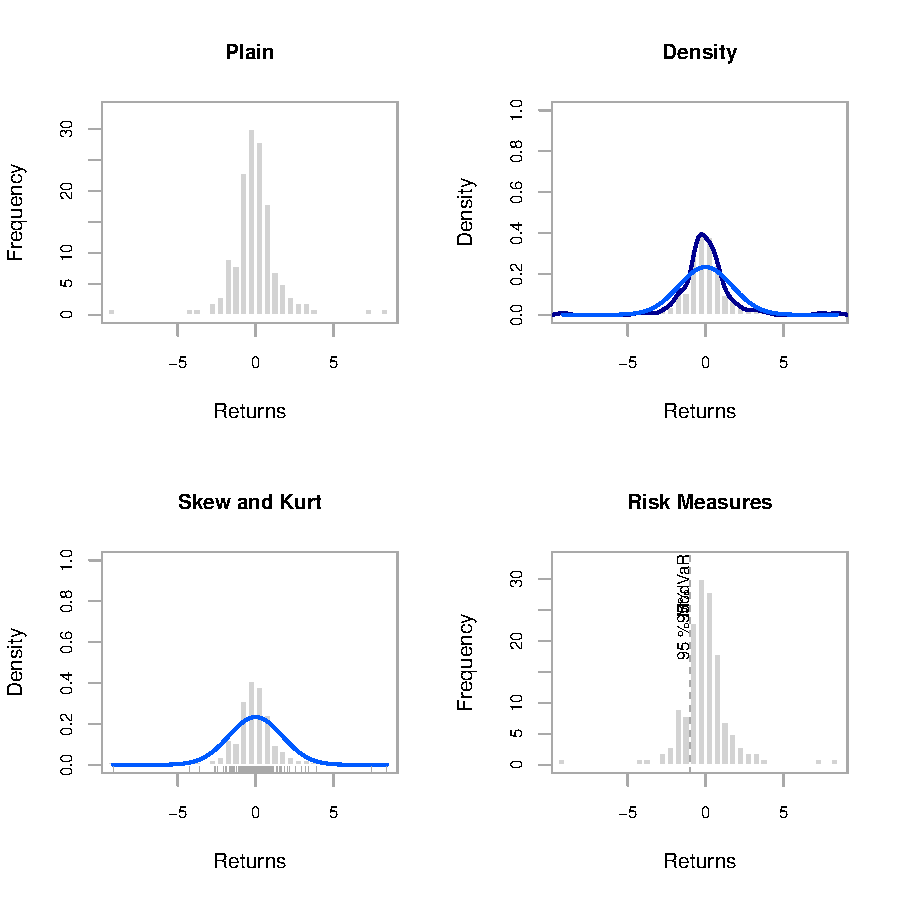
\includegraphics{OkunevWhite-Graph10}

The above figure shows the behaviour of the distribution tending to a normal IID distribution.For comparitive purpose, one can observe the change in the charateristics of return as compared to the orignal.
\begin{Schunk}
\begin{Sinput}
> library(PerformanceAnalytics)
> data(edhec)
> Returns = Return.Okunev(edhec[,1])
> layout(rbind(c(1, 2), c(3, 4)))
>  chart.Histogram(edhec[,1], main = "Plain", methods = NULL)
>  chart.Histogram(edhec[,1], main = "Density", breaks = 40,
+  methods = c("add.density", "add.normal"))
>  chart.Histogram(edhec[,1], main = "Skew and Kurt",
+  methods = c("add.centered", "add.rug"))
> chart.Histogram(edhec[,1], main = "Risk Measures",
+  methods = c("add.risk"))
> 
\end{Sinput}
\end{Schunk}
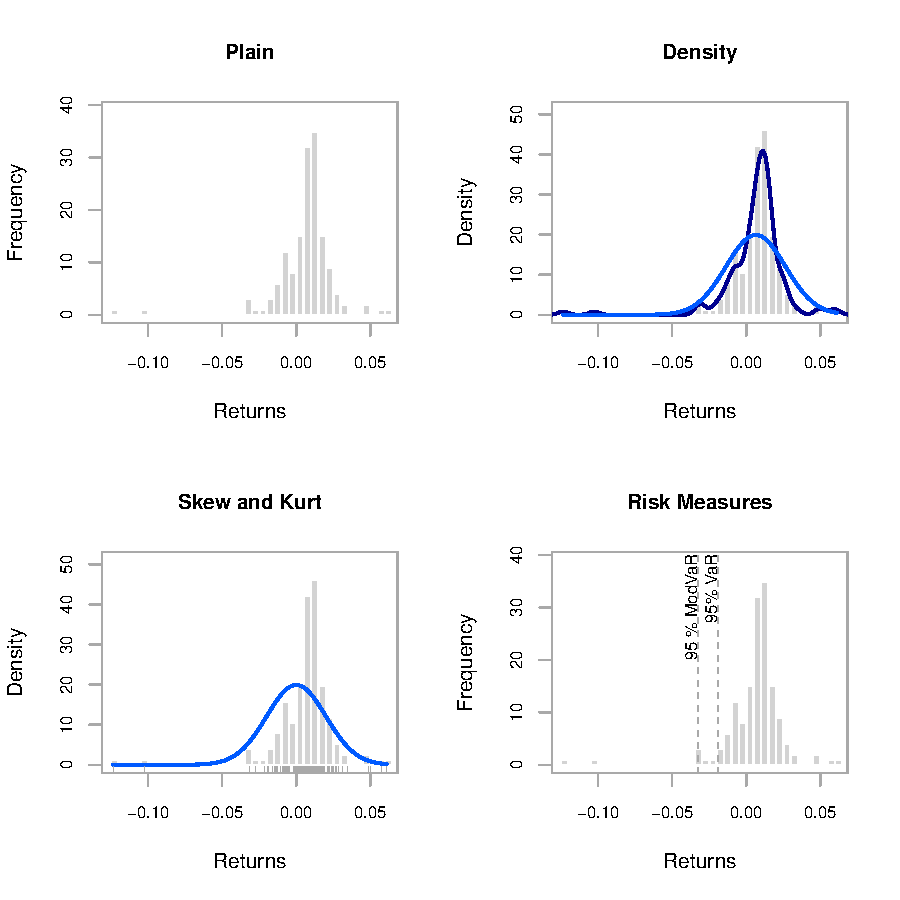
\includegraphics{OkunevWhite-Graph1}

\end{document}
